\documentclass[a4paper,10pt]{article}

\usepackage{tikz}
\usepackage{pgf}
\usetikzlibrary{arrows, calc, decorations.pathmorphing, shapes}

\usepackage[margin=3cm]{geometry}
\usepackage{adjustbox}
\usepackage[english]{babel}
\usepackage[latin1]{inputenc}
\usepackage{graphicx}
\usepackage{multirow}
\usepackage{makecell}
\usepackage{arydshln}
\usepackage{algorithm}
\usepackage[noend]{algpseudocode}
\usepackage{tikz}
\usetikzlibrary{shapes,arrows,shadows}
\usepackage[square,numbers]{natbib}
\usepackage{amsmath,amsfonts,amssymb,bm,dsfont,times}
\usetikzlibrary{positioning,calc,patterns}
\usepackage{hyperref}

\hypersetup{
  bookmarksnumbered,
  colorlinks=true,
  citecolor=blue,
  linkcolor=blue
}
\usepackage{caption}
\usepackage{subcaption}
\usepackage{textcomp}
\usepackage[toc,page]{appendix}
\definecolor{myred}{RGB}{255,66,56}
\pgfrealjobname{test}


\begin{document}
    
\pgfdeclarelayer{background}
\pgfdeclarelayer{foreground}
\pgfsetlayers{background,main,foreground}

\tikzstyle{sensor}=[draw, fill=blue!20, text width=3em,
    text centered, minimum height=2.5em,drop shadow]
\tikzstyle{sensor2}=[draw, fill=orange!20, text width=6em,
    text centered, minimum height=2.5em,drop shadow]
\tikzstyle{sensor3}=[draw, fill=orange, text width=4em,
    text centered, minimum height=2.5em,drop shadow]
\tikzstyle{ann} = [above, text width=5em, text centered]
\tikzstyle{wa} = [sensor, text width=5em, fill=red!20, inner sep=0pt,
    minimum height=4em, rounded corners, drop shadow]
\tikzstyle{sc} = [sensor, text width=13em, fill=red!20,
    minimum height=10em, rounded corners, drop shadow]

% Define distances for bordering
\def\blockdist{1.7}
\def\edgedist{0.5}

%-------------------------------------------------------------------------

\beginpgfgraphicnamed{pareto}
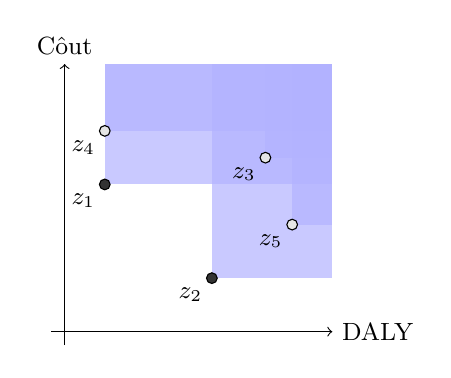
\begin{tikzpicture}[scale=1.7]
    \fill[fill=blue!30, opacity=0.7] (-0.7,0.1) rectangle (1,1);
    \filldraw[fill=black!80] (-0.7,0.1) circle (0.04) node [below left] {\small$z_1$};

    \fill[fill=blue!30, opacity=0.7] (0.1,-0.6) rectangle (1,1);
    \filldraw[fill=black!80] (0.1,-0.6) circle (0.04) node [below left] {\small$z_2$};

    \fill[fill=blue!30, opacity=0.7] (0.5,0.3) rectangle (1,1);
    \filldraw[fill=black!10] (0.5,0.3) circle (0.04) node [below left] {\small$z_3$};

    \fill[fill=blue!30, opacity=0.7] (-0.7,0.5) rectangle (1,1);
    \filldraw[fill=black!10] (-0.7,0.5) circle (0.04) node [below left] {\small$z_4$};

    \fill[fill=blue!30, opacity=0.7] (0.7,-0.2) rectangle (1,1);
    \filldraw[fill=black!10] (0.7,-0.2) circle (0.04) node [below left] {\small$z_5$};

    %\fill[fill=blue!30, opacity=0.7] (0.2,0.2) rectangle (1,1);
    %\fill[fill=white, opacity=1] (0.2,0.2) rectangle (0.5,0.7);

    \draw[->] (-1.1,-1)--(1,-1) node [right] {\small DALY}; 
    \draw[->] (-1,-1.1)--(-1, 1) node [above] {\small C\^out};
    %\draw (-1,-1) rectangle (1,1);
    %\node[] at (0.75,0.5) {\small $D_2$};
    %\node[] at (1.2,1.0) {\small $z^{\rm upp}$};
\end{tikzpicture}

\endpgfgraphicnamed

%---------------------------------------------------------------------------------------

\beginpgfgraphicnamed{pareto_1}
\begin{tikzpicture}[scale=1.7]
    \filldraw[fill=black!80] (-0.7,0.1) circle (0.04) node [below left] {\small$z_1$};

    \draw[->] (-1.1,-1)--(1,-1) node [right] {\small DALY}; 
    \draw[->] (-1,-1.1)--(-1, 1) node [above] {\small C\^out};
\end{tikzpicture}

\endpgfgraphicnamed

%---------------------------------------------------------------------------------------

\beginpgfgraphicnamed{pareto_2}
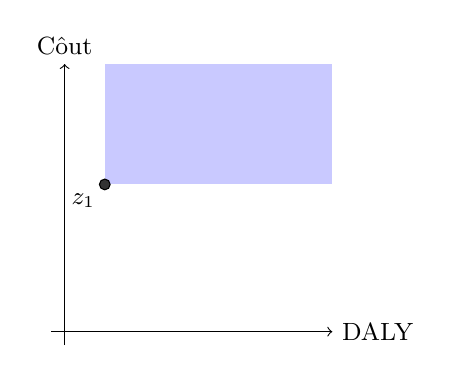
\begin{tikzpicture}[scale=1.7]
    \fill[fill=blue!30, opacity=0.7] (-0.7,0.1) rectangle (1,1);
    \filldraw[fill=black!80] (-0.7,0.1) circle (0.04) node [below left] {\small$z_1$};

    \draw[->] (-1.1,-1)--(1,-1) node [right] {\small DALY}; 
    \draw[->] (-1,-1.1)--(-1, 1) node [above] {\small C\^out};
\end{tikzpicture}

\endpgfgraphicnamed

%---------------------------------------------------------------------------------------

\beginpgfgraphicnamed{pareto_3}
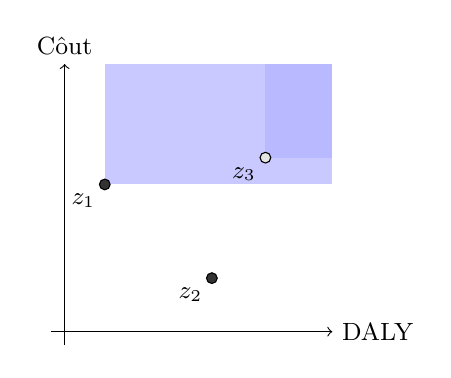
\begin{tikzpicture}[scale=1.7]
    \fill[fill=blue!30, opacity=0.7] (-0.7,0.1) rectangle (1,1);
    \filldraw[fill=black!80] (-0.7,0.1) circle (0.04) node [below left] {\small$z_1$};

    \fill[fill=blue!30, opacity=0.7] (0.5,0.3) rectangle (1,1);
    \filldraw[fill=black!10] (0.5,0.3) circle (0.04) node [below left] {\small$z_3$};
    	
    \filldraw[fill=black!80] (0.1,-0.6) circle (0.04) node [below left] {\small$z_2$};

    \draw[->] (-1.1,-1)--(1,-1) node [right] {\small DALY}; 
    \draw[->] (-1,-1.1)--(-1, 1) node [above] {\small C\^out};


\end{tikzpicture}

\endpgfgraphicnamed

%---------------------------------------------------------------------------------------

\beginpgfgraphicnamed{pareto_4}
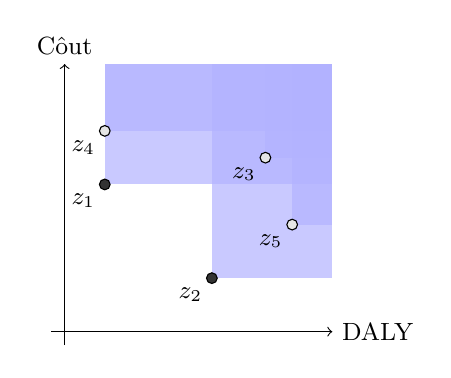
\begin{tikzpicture}[scale=1.7]
    \fill[fill=blue!30, opacity=0.7] (-0.7,0.1) rectangle (1,1);
    \filldraw[fill=black!80] (-0.7,0.1) circle (0.04) node [below left] {\small$z_1$};

    \fill[fill=blue!30, opacity=0.7] (0.1,-0.6) rectangle (1,1);
    \filldraw[fill=black!80] (0.1,-0.6) circle (0.04) node [below left] {\small$z_2$};

    \fill[fill=blue!30, opacity=0.7] (0.5,0.3) rectangle (1,1);
    \filldraw[fill=black!10] (0.5,0.3) circle (0.04) node [below left] {\small$z_3$};

    \fill[fill=blue!30, opacity=0.7] (-0.7,0.5) rectangle (1,1);
    \filldraw[fill=black!10] (-0.7,0.5) circle (0.04) node [below left] {\small$z_4$};

    \fill[fill=blue!30, opacity=0.7] (0.7,-0.2) rectangle (1,1);
    \filldraw[fill=black!10] (0.7,-0.2) circle (0.04) node [below left] {\small$z_5$};

    %\fill[fill=blue!30, opacity=0.7] (0.2,0.2) rectangle (1,1);
    %\fill[fill=white, opacity=1] (0.2,0.2) rectangle (0.5,0.7);

    \draw[->] (-1.1,-1)--(1,-1) node [right] {\small DALY}; 
    \draw[->] (-1,-1.1)--(-1, 1) node [above] {\small C\^out};
    %\draw (-1,-1) rectangle (1,1);
    %\node[] at (0.75,0.5) {\small $D_2$};
    %\node[] at (1.2,1.0) {\small $z^{\rm upp}$};
\end{tikzpicture}

\endpgfgraphicnamed

%---------------------------------------------------------------------------------------

\beginpgfgraphicnamed{pals}
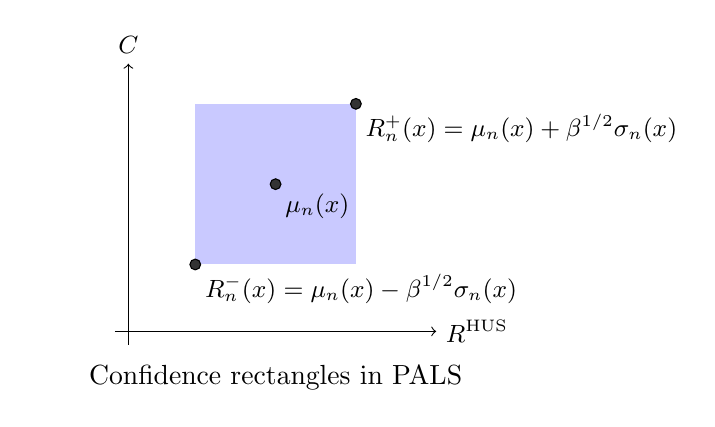
\begin{tikzpicture}[scale=1.7]
    
    \fill[fill=blue!30, opacity=0.7] (-0.5,-0.5) rectangle (0.7,0.7);
	\filldraw[fill=black!80] (-0.5,-0.5) circle (0.04) node [below right] {\small$R^{-}_n(x) 
	= \mu_n(x) - \beta^{1/2} \sigma_n(x)$};
    \filldraw[fill=black!80] (0.1,0.1) circle (0.04) node [below right] {\small$\mu_n(x)$};
    \filldraw[fill=black!80] (0.7,0.7) circle (0.04) node [below right] {\small$R^{+}_n(x)
	= \mu_n(x) + \beta^{1/2} \sigma_n(x)$};

    \draw[->] (-1.1,-1)--(1.3,-1) node [right] {\small$R^{\rm HUS}$}; 
    \draw[->] (-1,-1.1)--(-1, 1) node [above] {\small$C$};
    \node [below=0.3cm, align=flush center,text width=0.5\textwidth] at (0.1,-1)
        {
            Confidence rectangles in PALS
        };
\end{tikzpicture}

\endpgfgraphicnamed
%---------------------------------------------------------------------------------------

\beginpgfgraphicnamed{classify_p}
\begin{tikzpicture}[scale=0.9]

    %Draw axis
    \coordinate (y) at (0,5);
    \coordinate (x) at (5,0);
    %\draw[axis] (y) -- (0,0) --  (x);
    
    \draw[->] (0,0)--(5,0) node [right] {\small$R^{\rm HUS}$}; 
    \draw[->] (0,0)--(0,5) node [above] {\small$C$};

    %\node[below=1pt of {(5,0)}] {$R^{\rm HUS}$};
    %\node[left=1pt of {(0,5)}] {$C$};

        % Boxes
        \draw[dashed] (0.5,3.5) -- (0.5,4.5) -- (1.7,4.5) -- (1.7,3.5) -- cycle;
        \draw[dashed] (1,3) -- (1,3.8) -- (2,3.8) -- (2,3) -- cycle;
        \draw [line width=1pt] (3,2) -- (3,2.4) -- (3.4,2.4) -- (3.4,2) -- cycle;
	\fill[fill=green!30, opacity=0.7] (3,2) rectangle (3.4,2.4);
        \draw[dashed] (4,1) -- (4,2.2) -- (4.8,2.2) -- (4.8,1) -- cycle;
        \draw[dashed] (3.6,3) -- (3.6,3.8) -- (4.8,3.8) -- (4.8,3) -- cycle;

    %Coordinates of points
    \coordinate (y1) at (0.5,3.5);
    \coordinate (y2) at (1,3);
    \coordinate (y3) at (4,1);
    \coordinate (y4) at (3.6,3);

    \coordinate (y5) at (3.4,2.4);

    \coordinate (t1) at (1,1);
    \coordinate (t2) at (4,2.5);

    % Arrows
        \draw[<-,dotted] (y1) -- (t1);
        \draw[<-,dotted] (y2) -- (t1);
        \draw[<-,dotted] (y3) -- (t1);
        \draw[<-,dotted] (y4) -- (t1);

        \draw[<-,dotted] (y5) -- (t2);

        % Text
        \node[below=1pt of {t1}] {$R_n^{-}$};
        \node[right=1pt of {t2}] {$R_n^{+}(x)$};

    % Draw them
    \draw[draw=black,fill=black] (y1) circle [radius=0.025];
    \draw[draw=black,fill=black] (y2) circle [radius=0.025];
    \draw[draw=black,fill=black] (y3) circle [radius=0.025];
    \draw[draw=black,fill=black] (y4) circle [radius=0.025];

    \draw[draw=black,fill=black] (y5) circle [radius=0.025];

    \fill[gray!50,nearly transparent] (3,2) -- (3,2.4) -- (3.4,2.4) -- (3.4,2) -- cycle;
\end{tikzpicture}

\endpgfgraphicnamed
%---------------------------------------------------------------------------------------

\beginpgfgraphicnamed{classify_n}
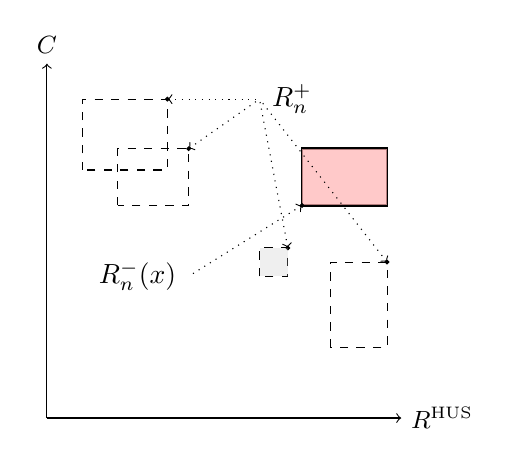
\begin{tikzpicture}[scale=0.9]

    %Draw axis
    \coordinate (y) at (0,5);
    \coordinate (x) at (5,0);
    %\draw[axis] (y) -- (0,0) --  (x);
    
    \draw[->] (0,0)--(5,0) node [right] {\small$R^{\rm HUS}$}; 
    \draw[->] (0,0)--(0,5) node [above] {\small$C$};

    %\node[below=1pt of {(5,0)}] {$R^{\rm HUS}$};
    %\node[left=1pt of {(0,5)}] {$C$};

        % Boxes
        \draw[dashed] (0.5,3.5) -- (0.5,4.5) -- (1.7,4.5) -- (1.7,3.5) -- cycle;
        \draw[dashed] (1,3) -- (1,3.8) -- (2,3.8) -- (2,3) -- cycle;
        \draw[dashed] (3,2) -- (3,2.4) -- (3.4,2.4) -- (3.4,2) -- cycle;
        \draw[dashed] (4,1) -- (4,2.2) -- (4.8,2.2) -- (4.8,1) -- cycle;
        \draw [line width=1pt] (3.6,3) -- (3.6,3.8) -- (4.8,3.8) -- (4.8,3) -- cycle;
	\fill[fill=red!30, opacity=0.7] (3.6,3) rectangle (4.8,3.8);

    %Coordinates of points
    \coordinate (y1) at (1.7,4.5);
    \coordinate (y2) at (2,3.8);
    \coordinate (y3) at (4.8,2.2);
    \coordinate (y4) at (3.4,2.4);

    \coordinate (y5) at (3.6,3);

    \coordinate (t1) at (3,4.5);
    \coordinate (t2) at (2,2);

    % Arrows
        \draw[<-,dotted] (y1) -- (t1);
        \draw[<-,dotted] (y2) -- (t1);
        \draw[<-,dotted] (y3) -- (t1);
        \draw[<-,dotted] (y4) -- (t1);

        \draw[<-,dotted] (y5) -- (t2);

        % Text
        \node[right=1pt of {t1}] {$R_n^{+}$};
        \node[left=1pt of {t2}] {$R_n^{-}(x)$};

    % Draw them
    \draw[draw=black,fill=black] (y1) circle [radius=0.025];
    \draw[draw=black,fill=black] (y2) circle [radius=0.025];
    \draw[draw=black,fill=black] (y3) circle [radius=0.025];
    \draw[draw=black,fill=black] (y4) circle [radius=0.025];

    \draw[draw=black,fill=black] (y5) circle [radius=0.025];

    \fill[gray!50,nearly transparent] (3,2) -- (3,2.4) -- (3.4,2.4) -- (3.4,2) -- cycle;
\end{tikzpicture}

\endpgfgraphicnamed

\end{document}
